% exp.tex
% 9/5/2013 jichi

\section{Experiment Results}
\label{sec-exp}
To evaluate the accuracy of our hot-spot communication predictions
  and the performance implications of our manually applied optimizations to better overlap computation with communication,
we applied our approach to model and optimize 7 MPI applications from the NAS NPB~\cite{npb}
  on two clusters shown in Figure~\ref{tab:hw}.
The first Intel platform is a large high-performance computing cluster with very fast internode communication through InfiniBand.
  The second platform is in a small data center where the internode communication is through relatively slow Ethernet.
Both clusters use MPICH 3.1.1~\cite{mpich2} as the underlying MPI library.
Because our current analytical performance model cannot estimate intranode MPI communication time,
  we have allocated a single MPI process per node on both clusters.
  % so that MPI communication is inter-node.
%\todo{
%  (jichi: note, for DISCO, it is on HP ProLiant BL460c Generation 6 (G6) Server Blade; for Blues, I only know it has an Intel server, but I didn't find a code name for its server).
%}
%\begin{itemize}
%\item Intel Xeon x86 cluster
%  with 2.6GHz processors interconnected using Infiniband. Benchmarks are compiled using ICC/Ifort 13.1.
%\item Intel Xeon x64 cluster (referred as Intel x64)
%  with 3.2GHz processors interconnected using 1 Gbps Ethernet.
%  Benchmarks are compiled using GCC/Gfortran 4.4.7.
%\end{itemize}
% Disco: https://www.google.com/search?q=disco+uccs&ie=utf-8&oe=utf-8
% Blues: http://www.lcrc.anl.gov/about/Blues
\begin{table}
\caption{Experiment platforms}
\begin{center}
\begin{tabular}{c|c c}
\hline
Server & Intel & HP ProLiant BL460c Gen6 \\
\hline
          &  Intel Xeon & Intel Xeon \\
Instruction set  &  x86 & x64 \\
Frequency &  2.6 GHz & 3.2 GHz \\
Compiler  &  ICC/Ifort 13.1 & GCC/Gfortran 4.4.7 \\
Network   &  InfiniBand Qlogic QDR & 1 Gbps Ethernet \\
% for disco, 24nodes are on 3 racks with 8 nodes on each rack
Total nodes &  301 & 24 on 3 racks\\
Maximum memory &  64 GB & 48 GB \\
%Hyperthread &  disabled & enabled \\
\hline
\hline
\end{tabular}
\end{center}
\label{tab:hw}
\end{table}

For each MPI application, we first used our extended SKOPE performance modeling framework to find the most time-consuming MPI communication in the application.
Then, we manually applied the computation-communication optimization to the enclosing loop surrounding the identified communications.
We measured the performance improvements from the optimizations using input data
 provided by the NPB benchmarks and using a range of 2 to 9 nodes for each application.
%which are 3/9 nodes for BT and SP,and 2/4/8 nodes for the others NPB applications.
%jichi: as I only had access to at most 10 nodes on DISCO that were not used by other people, I was not able to do experiment for more nodes.
%Here, BT/SP used different configurations since they required the number of nodes to be times of 3 instead of 2.
% What time is measured?
% how much is the variation?
% Average = 19 on blues and 18 on discos, and maximum is 88% in blues and 76 on discos
Besides using the built-in timers within the NPB applications to collect their overall performance,
  we manually instrumented the source code of the applications to report the performance of  individual communications.
%For each NPB application, we measure each configuration exact once instead of multiple times
%  since these applications are internally implemented to take multiple times of iterations to evaluate their communication kernels.
%Our results show that our optimizations is able to achieve on average 18.4\% and at most 88\% speed up.

%In order to evaluate the performance of the optimization framework,
%I used the framework to optimize MPI \texttt{NASA Parallel Benchmarks}, or \texttt{NPB}, and test the result code on BlueGene/Q.
%To answer these questions, I first design micro benchmarks to evaluate different distributions of MPI\_Test.
%Then, the hot spots identified by analytical modeling and tuning are compared.
%Finally, I applied the optimization approach to NAS Parallel Benchmarks~\cite{npb}.

%This section uses the results profiled on two clusters
%to verify the model-based hot-spot analysis and evaluate the overlap optimization.
%%Both of the clusters are Intel architecture.
%One of the clusters consists of Intel x86 machines from the Argonne National Laboratory,
%and the other one consists of Intel x86\_64 machines from the University of Colorado at Colorado Springs.

%%%%%%
\subsection{Accuracy of Hot Communication Prediction}

To evaluate the accuracy of our modeling of MPI communications,
  we compared the set of communication hot spots selected using our model with those found by profiling
  the NPB applications, using class B input on 4 nodes.
%\done{jichi: I also tested A/C for my first two applications (FT and IS). But I cannot declare this conclusion for all configurations for other NPB applications.}
The different hot-spot selection for the NPB applications are shown in Table~\ref{tab:npb:hot}.
When selecting the top time-consuming MPI communications, we required that their overall time be at least 80\% of the application's overall communication time.
In this case, our predictive modeling selected the same set of hot communications as found using application profiling.
%The table does not include NPB BT and NPB SP whose communication are non-blocking that cannot be profiled,
%  and it does not have the ranks for non-blocking \texttt{MPI\_Irecv} in NPB CG and NPB MG.
%Our modeling work successfully find all correct hot spots.
When asked to select a given number of the most time-consuming communications, however, the output by our predictive modeling differs by at most 2 selections compared with using profiling,
%  which could happen when certain hot communications have very similar communication time.
for the NAS LU benchmark.
Here the most time-consuming communications are pairs of sends/receives at four symmetric directions, which were estimated to take the same time by our predictive modeling.
However, their actual runtime collected through profiling differ by 37\%, because the execution of the processes is unbalanced, resulting in extra wait time to synchronize the corresponding MPI\_Send/MPI\_Recv operations.
Figure~\ref{fig:model:ft:B} compares our projected communication time with the actual measured time for NAS FT, using two and four processors.  Here in spite of the small error rates in projecting the absolute values of the communication time, our modeling framework was able to accurately capture the relative importances of the various communication operations.
%The X-axis represents the different hot communications in NAS FT;
%  the Y-axis on the left represents the actual total runtime of all selected hot spots,
%  and that on the right represents the their total estimated communication time using the LogGP model.
%Although the absolute values of the actual and estimated communication time could vary significant,
%  the relative time spent for different communications are very similar.

%\begin{figure}
%{\scriptsize
%\begin{subfigure}{.48\textwidth}
%\centering
%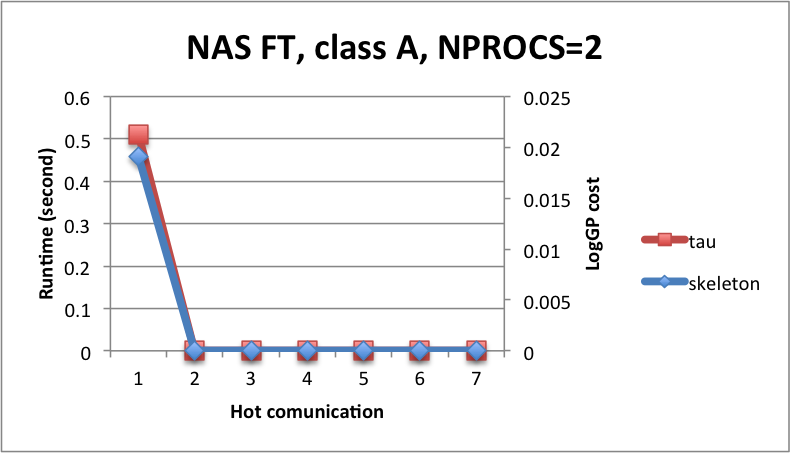
\includegraphics[width=.9\textwidth]{fig/blues/ft_A_2_model.png}
%\caption{Communication on 2 nodes}
%\label{fig:model:ft:A:2}
%\end{subfigure}
%\begin{subfigure}{.48\textwidth}
%\centering
%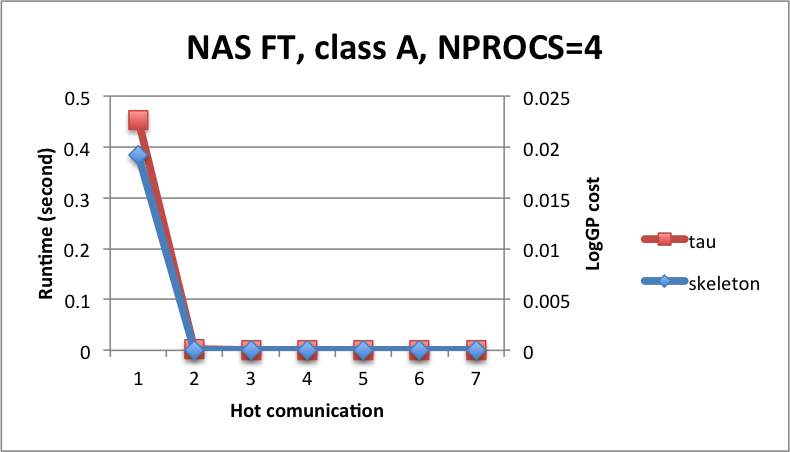
\includegraphics[width=.9\textwidth]{fig/blues/ft_A_4_model.png}
%\caption{Communication on 4 nodes}
%\label{fig:model:ft:A:4}
%\end{subfigure}
%\caption{Profiled runtime and modeled cost of NAS FT with small input (A) on x86 cluster}
%\label{fig:model:ft:A}
%}%\scriptsize
%\end{figure}

\begin{figure}
{\scriptsize
\begin{subfigure}{.48\textwidth}
\centering
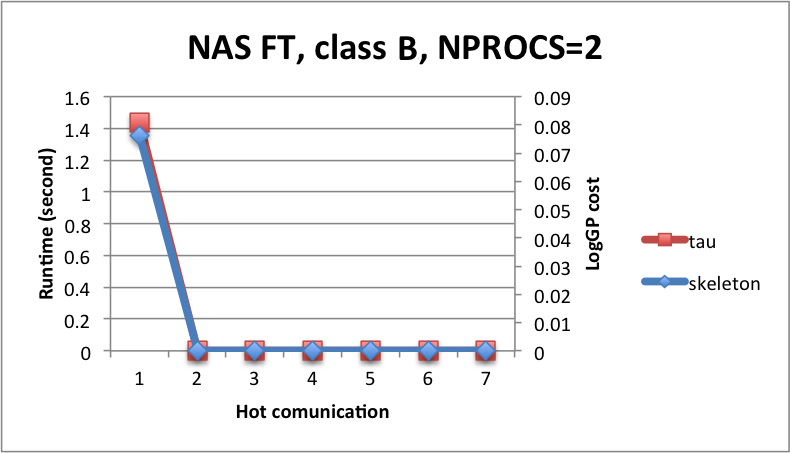
\includegraphics[width=.9\textwidth]{fig/blues/ft_B_2_model.png}
\caption{Communication on 2 nodes}
\label{fig:model:ft:B:2}
\end{subfigure}
\begin{subfigure}{.48\textwidth}
\centering
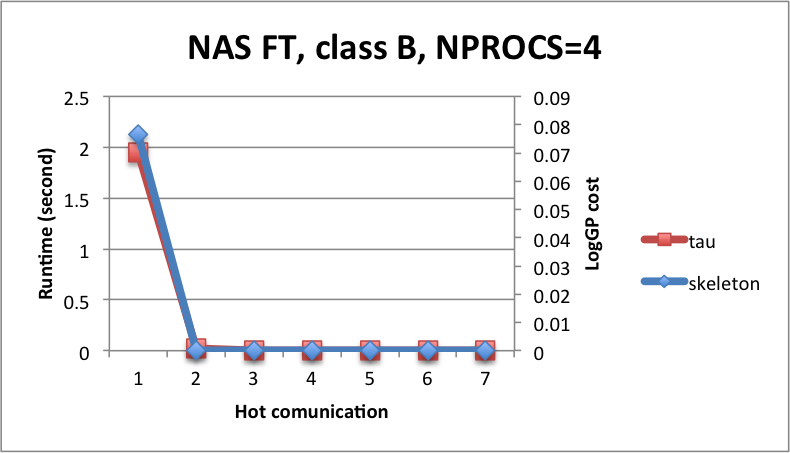
\includegraphics[width=.9\textwidth]{fig/blues/ft_B_4_model.png}
\caption{Communication on 4 nodes}
\label{fig::modelft:B:4}
\end{subfigure}
\caption{Profiled runtime and modeled cost of NAS FT with middle-sized input (B) on x86 cluster}
\label{fig:model:ft:B}
}%\scriptsize
\end{figure}
%As shown in Figure~\ref{fig:model:ft:A} and Figure~\ref{fig:model:ft:B},
%  our modeling approach identified the same hot communication as the tau profiler.
%The most time consuming MPI call is MPI\_Alltoall, which takes more than 90\% of the total communication time.

% NPB class = B, NPROCS = 4
\begin{table}
\caption{
Differences between the projected hot-spot selection and
the measured hot-spot selection based on profiling with 80\% threshold for class B data on 4 nodes. Zero means
the set of $N$ hot spots equals the top $N$ hot spots.
}%\caption
%{\scriptsize
\begin{center}
\begin{tabular}{c|r|r|r|r|r|r|r|r}
\hline
&\multicolumn{7}{c}{Selected number of hot MPI communications}\\
        & 1 & 2 & 3 & 4 & 5 & 6 & 7 & 8 \\
\hline
FT      & 0 &   &   &   &   &   &   &   \\  % 1:MPI_Alltoall, 99%
IS      & 0 & 0 &   &   &   &   &   &   \\  % 1:MPI_Alltoallv = 3.494, MPI_Allreduce = 1.279
CG      & 0 &   &   &   &   &   &   &   \\  % 1:MPI_Send 6,383, 2:MPI_Irecv
LU      & 0 & 1 & 2 & 2 & 1 & 1 & 0 & 0 \\  % MPI_Send
MG      & 1 & 1 & 0 & 1 & 1 & 0 &   &   \\  % MPI_Send
\hline
\hline
\end{tabular}
\end{center}
%}%\scriptsize
\label{tab:npb:hot}
\end{table}

%\begin{figure}
%{\scriptsize
%\centering
%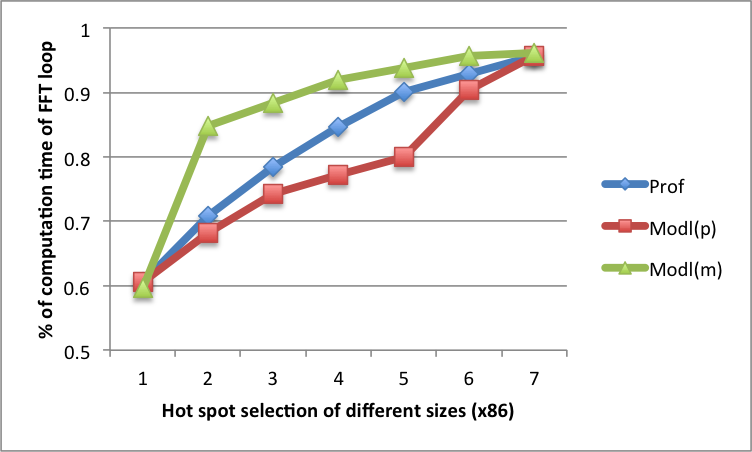
\includegraphics[width=.48\textwidth]{fig/blues/ft_B_4_hotspot.png}
%\caption{
%Profiled and modeled computation time of NAS FT's overlap region (the FFT loop) with middle-sized input (B) on 4 x86 nodes.
%{\tt Prof} and {\tt Modl} refer to the hot spot
%selections resulted from BG/Q profiling and performance modeling.
%{\tt Modl(p)} and {\tt Modl(m)} show the projected and measured
%runtime coverage on x86 cluster using the model-projected hot spots, respectively.
%}%\caption
%\label{fig:hot:ft}
%}%\scriptsize
%\end{figure}

%\begin{table}
%%{\scriptsize
%\begin{center}
%\begin{tabular}{c|r r r r r r r}
%\hline
%&\multicolumn{7}{c}{Sizes of local hot spot selections}\\
%        & 1 & 2 & 3 & 4 & 5 & 6 & 7 \\
%\hline
%FT      & 0 & 1 & 1 & 1 & 2 & 1 & 0 \\
%\hline
%\hline
%\end{tabular}
%\end{center}
%%}%\scriptsize
%\caption{
%\IPDPS{Differences between the projected hot spot selection and
%the measured hot spot selection based on profiling. Zero means
%the set of $N$ hot spots equals the top $N$ hot spots.
%%Q.{\tt Modl} and X.{\tt Modl} refer to hot spot selections for
%%BG/Q and Xeon based on our modeling, respectively.
%%Q.{\tt Xeon} refers to hot spot selection for BG/Q based on Xeon profiling.
%%X.{\tt BG/Q} refers to hot spot selection for Xeon based on BG/Q profiling.
%}
%}%\caption
%\label{tab:hot:ft}
%\end{table}

\subsection{Impact of Optimizations}
%\begin{figure}
%{\scriptsize
%\centering
%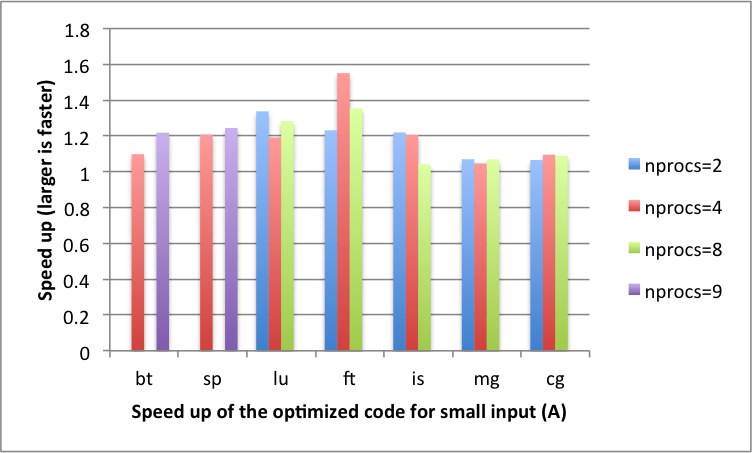
\includegraphics[width=.8\textwidth]{fig/disco/npb_disco_A.png}
%\caption{Speed up of NPB with input A class}
%\label{fig:npb:A}
%}%\scriptsize
%\end{figure}
\begin{figure}
{\scriptsize
\centering
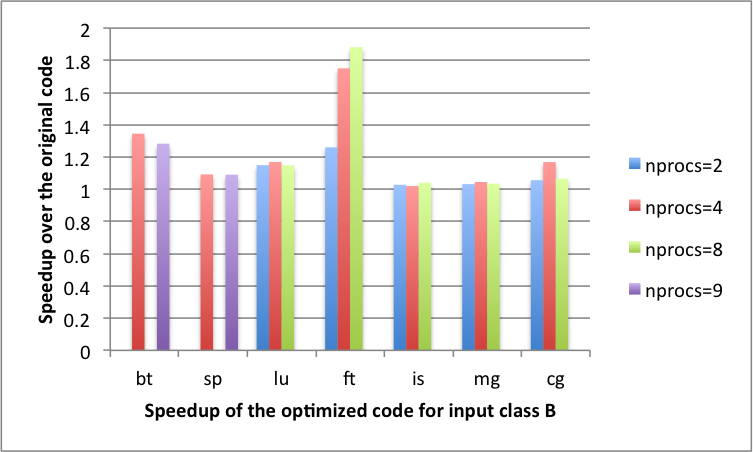
\includegraphics[width=.48\textwidth]{fig/blues/npb_blues_B.png}
\caption{Optimization speedups on the InfiniBand cluster.}
\label{fig:npb:x86}
}%\scriptsize
\end{figure}
\begin{figure}
{\scriptsize
\centering
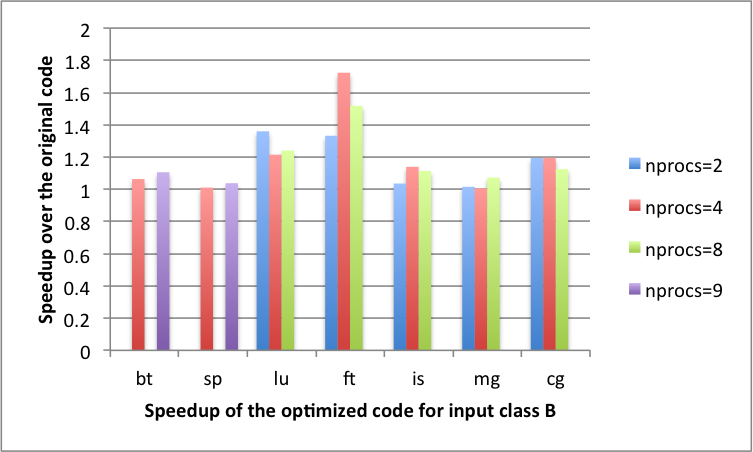
\includegraphics[width=.48\textwidth]{fig/disco/npb_disco_B.png}
\caption{Optimization speedups on the Ethernet cluster.}
\label{fig:npb:x64}
}
\end{figure}
%\begin{figure}
%{\scriptsize
%\centering
%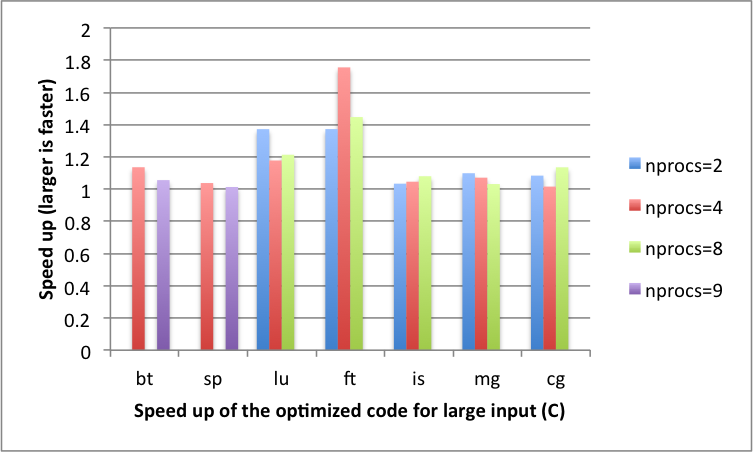
\includegraphics[width=.8\textwidth]{fig/disco/npb_disco_C.png}
%\caption{Speed up of NPB with input C class}
%\label{fig:npb:C}
%}%\scriptsize
%\end{figure}


Figures~\ref{fig:npb:x86} and \ref{fig:npb:x64}
show the speedups we attained by enabling better computation-communication overlapping for the NPB applications.
In particular, for each benchmark, the performance of the original application and the optimized code is measured by using input class B on 2, 4, 8, and 9 nodes,  with one MPI process bound to each node, 
with the exception of NAS BT and SP, which require the number of processes to be a multiple of 3 and so are configured to run on 3 and 9 nodes only.
The overall elapsed time of each application is measured by using NPB's built-in timer, which reports the elapsed time of multiple iterations with the exclusion of the initialization time.


Among all the NPB applications, FT and IS are the only benchmarks that use {\em alltoall} collectives as the main communication operation; the other benchmarks mostly use point-to-point send/receives.
Our optimization attained 3--88\% speedup for all applications.
The maximum 88\% performance improvement is observed with the NAS FT benchmark, which uses a time-consuming $MPI\_Alltoall$ operation, enclosed inside the outermost loop of the application,  to exchange a large amount of data.
The lowest speedup (3\%) is observed with NAS MG, which does not have sufficient local computation in the surrounding loop of the MPI communication to overlap with communication. \todo { I think we need to discuss more the difference between using the two different platforms}

%Another application NAS IS has the similar structure whose main loop is also the same as its communication loop.
%However, its most time-consuming communication is $MPI\_Alltoallv$ and the sizes of the communication data vary a lot at runtime.
%Depending on the input, the communication time of each $MPI\_Alltoallv$ call could be very short so that it is not able to hide the computation.
%As the result, our optimization is not able to achieve the same speedup as NAS FT.
%% 2. not single most consuming communication but multiple: lu, cg, bt, sp
%% MPI send/recv instead of alltoall.
%For NPB applications other than NAS FT and IS,
%  the majority of the communication time is spent on point-to-point send/receive instead of single alltoall collective calls.
%In these applications, there are communication calls that are not in loops, which we are not able to optimize.
%And the communication loops that we try to optimize are smaller than the main loop in these applications.
%As the result, not all computation is overlapped with the communication which result in less speedup.
% 3. Slowest mg, computation hot spot is out of communication loop
% The structure of MG is like this:
%   Loop
%     Loop -- the loop with interleaved computation/communication that we optimized
%       MainCommunication -- overlapped
%       VeryLittleComputation -- overlapped
%     MajorComputation -- not overlapped
%   Reduce -- final reduce outside of main loop that is also not overlapped


% EOF

%\subsubsection{NAS FT and IS}
%The most-time consuming communications are single all2all blocking collectives in the main loop,
%  and there is no overlapping of computation and communication at all in the original source code.
%Our optimization first converts blocking collectives to non-blocking versions,
%  and then reorders them to achieve overlap.
%Our optimization achieved the most speedup in NAS FT,
%  where the communication is $MPI\_Alltoall$
%  that always exchanges large amount of data.
%For NAS IS,
%   the most time-consuming communication IS is $MPI\_Alltoallv$ and the sizes of the data being communicated vary from less than 10 to as large as 30k.
%The communication time and computation time for IS is not always comparable.
%As the result, our optimization to overlap computation and communication saves more time for FT than for IS.
%
%\subsubsection{NAS BT and SP}
%The communications are done through non-blocking p2p send and receive in a group of $MPI\_Isend$, $MPI\_Irecv$, and $MPI\_Waitall$,
%  where the communications themselves in the same loop have already been overlapped.
%We first outline the consequent $MPI\_Isend$ and $MPI\_Irecv$ into the $Icomm(I)$ function and move $MPI\_Waitall$ into the $Wait(I)$ function,
%  and then reorder these communication with the nearby computation in the same loop to overlap them.
%Since the original communications are already non-blocking,
%  there is no need to convert the blocking communications to non-blocking versions.
%Comparing to FT and IS,
%  because the overlapped p2p communication exchanges less data and takes shorter time,
%  the overlap optimization achieves less speedup.
%
%\subsubsection{NAS MG, CG, and LU}
%The communications are done through pairs of blocking send and non-blocking receive ($MPI\_Send$, $MPI\_Irecv$, and $MPI\_Wait$),
%  but there is no overlapping of computation and communication in the original implementation.
%In our optimization, we first convert $MPI\_Send$ to $MPI\_Isend$ with $MPI\_Wait$,
%  then outline the $MPI\_Isend$ and $MPI\_Irecv$ into the $Icomm(I)$ function and their $MPI\_Wait$ into the $Wait(I)$ function,
%  and at last reorder these communication with the nearby computation in the same loop to achieve overlap.
%The structures of the optimized communication loops in CG and MG are similar,
%  where the communication takes much more time than the computation in the same loop.
%% jichi: MG and CG are like this
%% Loop:
%%   some computation -- not overlapped
%%   Loop:
%%     some computation  -- overlapped
%%     hot communication
%%   some computation -- not overlapped
%Additionally, some computation hot spots are not in the communication loop and not overlapped as the result,
%  which limit our overall speedup of our CCO optimization.
%In comparison, LU achieves better speedup,
%  where the hot communication takes less time than the computation in the same loop
%  and hence the communication latency can be fully hidden in the computation time.

%\subsubsection{Load balance}
%
%\begin{figure}
%{\scriptsize
%\centering
%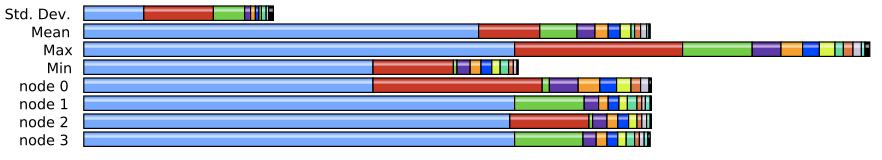
\includegraphics[width=.9\textwidth]{fig/blues/ft_B_4_tau.png}
%\caption{Runtime of NAS FT with middle-sized input (B) on 4 x86 nodes}
%\label{fig:opt:ft:B}
%}%\scriptsize
%\end{figure}
%
%\begin{figure}
%{\scriptsize
%\centering
%\includegraphics[width=.9\textwidth]{fig/blues/is_B_4_tau.png}
%\caption{Runtime of NAS IS with middle-sized input (B) on 4 x86 nodes}
%\label{fig:opt:ft:B}
%}%\scriptsize
%\end{figure}
%
%\begin{figure}
%{\scriptsize
%\centering
%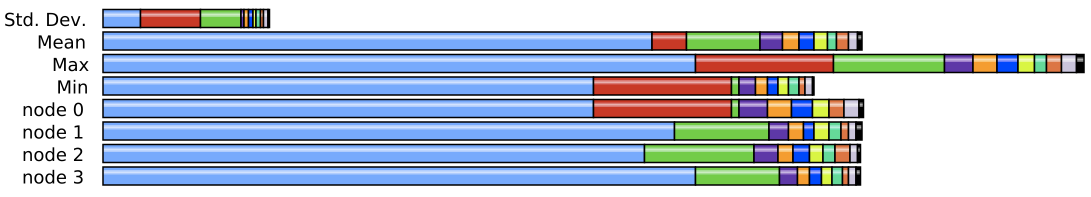
\includegraphics[width=.9\textwidth]{fig/disco/ft_B_4_tau.png}
%\caption{Runtime of NAS FT with middle-sized input (B) on 4 x86\_64 nodes}
%\label{fig:opt:ft:B}
%}%\scriptsize
%\end{figure}
%
%\begin{figure}
%{\scriptsize
%\centering
%\includegraphics[width=.9\textwidth]{fig/disco/is_B_4_tau.png}
%\caption{Runtime of NAS IS with middle-sized input (B) on 4 x86\_64 nodes}
%\label{fig:opt:ft:B}
%}%\scriptsize
%\end{figure}
%\subsection{Insertion of MPI\_Test}
%\begin{figure}
%\centering
%{\scriptsize
%\begin{verbatim}
%Loop J = 1 ... M
%  MPI_Ialltoall
%  Loop I = 1 ... N
%    If I % Freq == 0
%      MPI_Test
%    nanosleep
%  MPI_Wait
%\end{verbatim}
%\caption{The micro benchmark used to test distribution of MPI\_Test}
%\label{fig:cco_test}
%}%\scriptsize
%\end{figure}
%\begin{table}
%{\scriptsize\centering
%\begin{tabular}{|l|l|l|} \hline
%Distribution    & Time (sec) & Descriptions \\
%\hline
%orig            & 5.424621  & original benchmark without overlapping \\
%orig-comm       & 2.224972  & total communication time of the original code \\
%orig-comp       & 3.2       & total computation time of the original code \\
%5-test          & 3.56385   & evenly insert 5 MPI\_Test \\
%8-test          & 3.229617  & evenly insert 8 MPI\_Test \\
%10-test         & 3.15611   & evenly insert 10 MPI\_Test \\
%16-test         & 3.249664  & evenly insert 16 MPI\_Test \\
%100-test        & 3.590359  & evenly insert 100 MPI\_Test \\
%1000-test       & 17.265191 & evenly insert 1000 MPI\_Test \\
%unevel1-10-test & 3.939304  & unevenly first insert 8 slow and 2 fast MPI\_Test \\
%unevel2-10-test & 3.624152  & unevenly first insert 2 slow and 8 fast MPI\_Test \\
%\hline
%\end{tabular}
%}%\scriptsize
%\caption{Micro benchmark of overlapped MPI\_Alltoall}
%\label{tab:mpitest}
%\end{table}
%\begin{figure}
%{\scriptsize
%\centering
%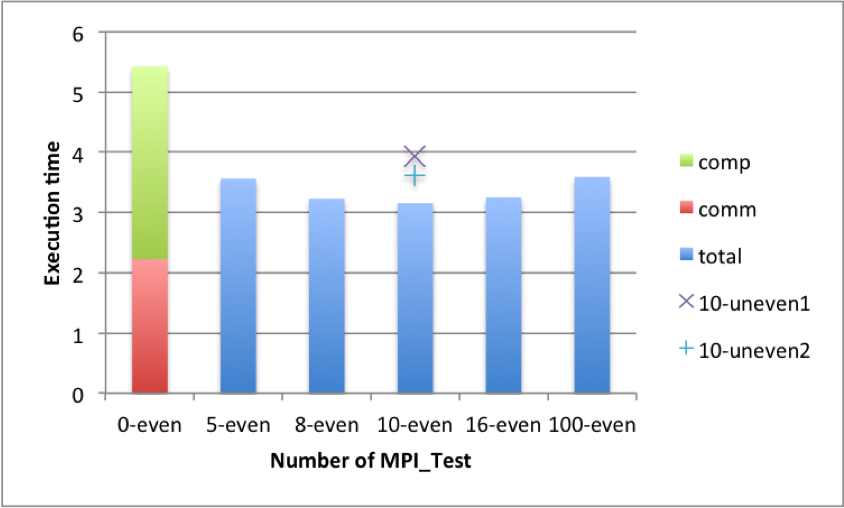
\includegraphics[width=.48\textwidth]{fig/mpitest.png}
%\caption{Micro benchmark of overlapped MPI\_Alltoall}
%\label{fig:exp:mpitest}
%}%\scriptsize
%\end{figure}
%To evaluate the impact of MPI\_Test distribution to the overlapping of computation and communication,
%  we designed a micro benchmark as shown in Figure~\ref{fig:exp:mpitest}.
%It contains a single loop of MPI\_Alltoall,
%  and a loop of computation emulated using $nanosleep()$.
%The execution time is shown in Figure~\ref{fig:exp:mpitest} and Table~\ref{tab:mpitest}.
%We tried different numbers of MPI\_Test when even distributed,
%  which shows the 10 MPI\_Test configuration has the best performance,
%  and the execution is monotoned increasing when the number of MPI\_Test is increasing or decreasing.
%This implies the best MPI\_Test frequency can be tuned through binary search.
%Given 10 MPI\_Test,
%  we also tried non-evenly distributed cases of \texttt{unevel1-10-test} and \texttt{uneven2-10-test},
%  where the sleep time between 2 MPI\_Test is will be 4 times slower than the sleep time between the other 8 MPI\_Test.
%Both the non-evenly distribution cases are slower than the evenly distributed MPI\_Test.
%NAS DT (Data Traffic) and EP (Embarrassingly Parallel) are excluded, which cannot benefit from our optimization approach.
